\section{Punto de Vista de Proceso de Negocio}

El punto de vista del proceso de negocio, es en donde se definen los procesos organizacionales del proyecto, es decir, lo que se convertirá en el paradigma alrededor del cual la organización resuelve toda su misión, sus funciones, objetivos. En concreto es el Core en donde se determina la funcionalidad organizacional.
Este punto de vista contribuye al entendimiento real de lo que se requiere con el proyecto, es decir, su objetivo organizaciones, todo desde un punto de vista administrativo, dando una visión más amplia y completa a lo que se refiere con la finalidad del proyecto.

\subsection{Modelo de Proceso de Negocio}
\begin{figure}[h!]
	\centering
	\includegraphics[width=.8\linewidth]{imgs/modelo/ProcesoNegocio}
	\caption{Modelo Proceso de Negocio}
\end{figure}

El modelo para el punto de vista de proceso de negocio, se centra en un proceso o función que como su nombre lo indica es el desarrollo del objetivo qu se requiere, asimismo cuenta con una serie de eventos de negocio los cuales anteceden y preceden al proceso de negocio, de la misma manera, está conformado por servicios, objetos y representaciones, además de definir el rol del proceso y el actor que interviene en el mismo.

\clearpage
\subsection{Caso  de Proceso de Negocio}
\begin{figure}[h!]
	\centering
	\includegraphics[width=.9\linewidth]{imgs/caso/negocio/ProcesoNegocio}
	\caption{Caso Proceso de Negocio}
\end{figure}

En el caso de nuestro proyecto, el proceso principal es el acompañamiento vocacional, vinculado al gran objetivo de propender por una educación inclusiva y dos eventos de negocio muy importantes que anteceden y preceden al proceso de negocio, el evento que antecede a este proceso de negocio es la culminación de la secundaria, posteriormente interviene el proceso de negocio con el acompañamiento vocacional y precede a este el evento de negocio del perfilamiento vocacional como finalización a este proceso, además este proceso principal está acompañado de tres subprocesos que en orden correspondiente son, en primer lugar la caracterización poblacional, continua con la identificación vocacional y finaliza con una retroalimentación.